\section{Implementación  de Funcionalidades}

Una vez que terminado el modelo del problema, el siguiente paso fue comenzar a implementar la base de datos. Es decir generar en RethinkDB las distintas tablas, documentos y consultas necesarias para resolver el problema.\\

Para ello creamos un pequeño programa que genere de manera aleatoria todos los datos necesarios, asegurándose de ser consistente al momento de crear documentos para los enfrentamientos, campeonatos, escuelas y demás. Ya que, por ejemplo, si un competidor gana un enfrentamiento, el mismo debe ser contabilizado en el Documento $Campeonato$.\\ \\

Una vez llenadas las tablas con los suficientes datos, implementamos cada una de las consultas:\\ \\

\begin{itemize}

\item{\textbf{Cantidad de enfrentamientos ganados por competidor para un campeonato dado.}

Como esta consulta debe realizarse para un Campeonato determinado, el primer paso es filtrar la tabla $Campeonatos$ hasta obtener el documento indicado. Para ello utilizamos la función $filter$ sobre el campo $anio$ que, por lo visto anteriormente, identifica inequívocamente a cada Campeonato.\\

Una vez seleccionado el campeonato, hicimos un concatMap y un reduce sobre todos los pares $(competidor,enfrentamientosGanados)$ de todas las escuelas que participan del campeonato, obteniendo así los datos necesarios para esta consulta.

\begin{verbatim}

r.db('TP2').table('Campeonato').filter({anio: 2017})("escuelas").concatMap(function(elem){
  	return elem("competidores");
  })
  .reduce(function(left, right){
    return left.add(right);
  })

\end{verbatim}
}

\item{\textbf{Cantidad de medallas por nombre de escuela en toda la historia}

Usando la función map, podemos tomar cada documento $Escuela$ y devolver únicamente los campos que nos interesan para resolver la consulta, es decir, su $nombreEscuela$ y la sumatoria de todos los campos $cantidadMedallas$ que se encuentren en el arreglo $medallasPorCampeonato$.

\begin{verbatim}

r.db("TP2").table("Escuela").map(
function(elem){
  return {id: elem("idEscuela"),nombre: elem("nombreEscuela"),
    		cantidadTotal: elem("medallasPorCampeonato").sum("cantidadMedallas")};
	}
)

\end{verbatim}
}

\item{\textbf{Para cada escuela, el campeonato donde gan\' m\'as medallas}

De forma similar a la consulta anterior usamos una función $map$. La cual devolverá, $nombreEscuela$ junto con el an\~o del campeonato cuya tupla $(anio,cantidadMedallas)$ asociada sea máxima. Es decir, corresponda al elemento de $medallasPorCampeonato$ con mayor cantidad de medallas.

\begin{verbatim}

r.db("TP2").table("Escuela").map(
  function(elem){
    var res = elem("medallasPorCampeonato").max("cantidadMedallas");
    return {escuela: elem("nombreEscuela"), campeonato: res("anio")};
  })

\end{verbatim}
}

\item{\textbf{Los arbitros que participaron en al menos 4 campeonatos}

Como cada documento $Arbitro$ contiene una lista con los an\~os de los campeonatos en los que participo, responder esta consulta significa filtrar aquellos árbitros que cumplan con la condición. Esto lo podemos hacer usando un $filter$ sobre el largo del arreglo $participoEn$, y devolviendo solo aquellos que tengan longitud mayor o igual a 4. 

\begin{verbatim}


r.db("TP2").table("Arbitro").filter(
function(elem){
  return elem("participoEn").count().ge(4);
})

\end{verbatim}
}

\item{\textbf{Las escuelas que han presentado el mayor numero de competidores en cada campeonato}

Usando un map podemos tomar cada campeonato, y como cada uno tiene asociado un arreglo con todas las escuelas, que a su vez contiene una lista con todos los competidores, podemos entonces responder a la consulta tomando el largo del arreglo de competidores, y comparándolo con las otras escuelas.

\begin{verbatim}


r.db('TP2').table('Campeonato').map(
  function(elem){

    var max = elem("escuelas").max(
      function(esc){
        return esc("competidores").count();
      })("competidores").count();
    
    return {anio: elem("anio"), escuelas: elem("escuelas").filter(
      function(val){
      	return val("competidores").count().eq(max)
      }).pluck("idEscuela","nombreEscuela")};
})

\end{verbatim}
}

%%%%%%%%%% Puede ser que haya que modificarla, la pongo por las dudas

\item{\textbf{Obtener los competidores que m\'as medallas obtuvieron por modalidad}

En esta consulta usaremos un map reduce. La idea es: en el map tomar a cada competidor y devolver una tupla con los campos $(idCompetidorSalto,maxMedallasSalto,idCompetidorCombate,maxMedallasCombate,...)$ inicializandolos con su respectivo id, y con las cantidades de medallas en cada categoría (las cuales están almacenadas en cada competidor). Luego, en el reduce, comparamos dichos valores y modificamos el idDelCompetidor según sea necesario. En pseudocodigo:

\begin{verbatim}
map(competidor)
	return ("1",<dni,numMedallasCombate,dni,numMedallasSalto,
			dni,numMedallasFormas,dni,numMedallasRotura>)
			
reduce(c,[tupla1,tupla2,...])
	
	idCompMaxSalto = tupla1.idCompetidorSalto;
	idCompMaxCombate = tupla1.idCompetidorCombate;
	 . . . . 
	idCompMaxRotura = tupla1.idCompetidorRotura;
	
	maxMedallasSalto = tupla1.maxMedallasSalto;
	 . . . .
	maxMedallasRotura = tupla1.maxMedallasRotura;
	
	for all tuplas t in [tupla1,tupla2,...] do
	   maxMedallasSalto = MAX(maxMedallasSalto,
								t.maxMedallasSalto);          
	   if (maxMedallasSalto < t.maxMedallasSalto)
			idCompMaxSalto = t.idCompetidorSalto;
	   
	   . . .
	   maxMedallasRotura = MAX(maxMedallasRotura,
								t.maxMedallasRotura);          
	   
	endFor						
	
	return <c,(idCompMaxSalto,maxMedallasSalto,...,idCompMaxRotura,maxMedallasRotura)>


\end{verbatim}

Y la consulta en rethinkDB ser\'ia:\\ \\

\begin{verbatim}

r.db('TP2').table('Competidor').
map(function(Comp){
  return 
    {"idCompSalto":Comp("dni"),
      "maxMedallasSalto":Comp("numMedallasSalto"),
      
     "idCompCombate":Comp("dni"),
      "maxMedallasCombate":Comp("numMedallasCombate"),
     
      "idCompFormas":Comp("dni"),
      "maxMedallasFormas":Comp("numMedallasFormas"),
      
     "idCompRotura":Comp("dni"),
      "maxMedallasRotura":Comp("numMedallasRotura"),
      
      "idCompEquipos":Comp("dni"),
      "maxMedallasEquipos":Comp("numMedallasEquipos"),
      };
}).
reduce(function(left, right) {
  return {
    idCompSalto:r.branch(left("maxMedallasSalto").ge(right("maxMedallasSalto")),
      left("idCompSalto"),right("idCompSalto")),
    maxMedallasSalto:r.branch(left("maxMedallasSalto").ge(right("maxMedallasSalto")),
      left("maxMedallasSalto"),right("maxMedallasSalto")),
    
    idCompCombate:r.branch(left("maxMedallasCombate").ge(right("maxMedallasCombate")),
      left("idCompCombate"),right("idCompCombate")),
    maxMedallasCombate:r.branch(left("maxMedallasCombate").ge(right("maxMedallasCombate")),
      left("maxMedallasCombate"),right("maxMedallasCombate")),
    
    idCompFormas:r.branch(left("maxMedallasFormas").ge(right("maxMedallasFormas")),
      left("idCompFormas"),right("idCompFormas")),
    maxMedallasFormas:r.branch(left("maxMedallasFormas").ge(right("maxMedallasFormas")),
      left("maxMedallasFormas"),right("maxMedallasFormas")),
    
    idCompRotura:r.branch(left("maxMedallasRotura").ge(right("maxMedallasRotura")),
      left("idCompRotura"),right("idCompRotura")),
    maxMedallasRotura:r.branch(left("maxMedallasRotura").ge(right("maxMedallasRotura")),
      left("maxMedallasRotura"),right("maxMedallasRotura")),
    
    idCompEquipos:r.branch(left("maxMedallasEquipos").ge(right("maxMedallasEquipos")),
      left("idCompEquipos"),right("idCompEquipos")),
    maxMedallasEquipos:r.branch(left("maxMedallasEquipos").ge(right("maxMedallasEquipos")),
      left("maxMedallasEquipos"),right("maxMedallasEquipos"))
  }
}
    );

\end{verbatim}
}

\end{itemize}

\subsection{Sharding}

Tomamos la tabla de Competidores, pues es la que tiene mayor cantidad de registros (alrededor de 2000), y creamos 3 shards. Inicialmente la base de datos particion\'o el total de los registros en un shard con 672 registros, el segundo con 621 y el tercero con 561. Luego realizamos inserciones de a 100 competidores y obtuvimos los siguientes resultados: \\ \\

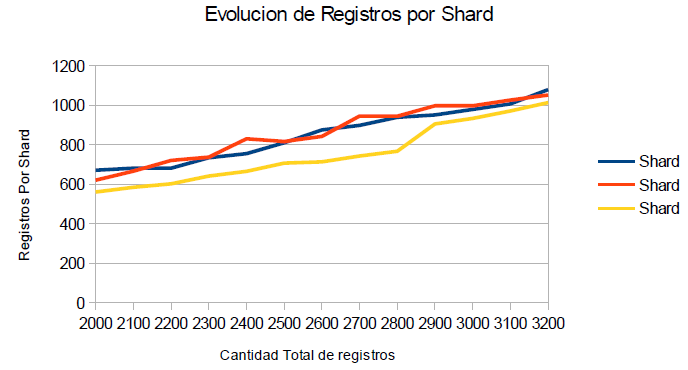
\includegraphics[scale=0.75]{Shards.png}

Como podemos ver en el grafico, rethinkDB distribuye equitativamente las inserciones a todos los shards, de manera de aliviar la carga de la base de datos al momento de responder consultas o realizar operaciones como inserciones.

